\chapter{Theoretical background}\label{background}

In this chapter we will provide the necessary background for the user to
understand the mechanisms used later in the paper. The description of the
following systems is a brief introduction, intended to familiarize the reader
with concepts that are fundamental for the methods presented.

Specifically, section \ref{sec:gzip} describes the functionality of the gzip
compression method and the algorithms that it entails. Section
\ref{sec:sameorigin} covers the same-origin policy that applies in the web
application security model. In section \ref{sec:tls} we explain the Transport
Layer Security, which is the main protocol used today to provide communications
security over the Internet. Finally, in section \ref{sec:mitm} we describe
attack methodologies in order for an adversary to perform a Man-in-the-middle
attack, such as ARP spoofing and DNS poisoning.

\section{gzip}\label{sec:gzip}

gzip is a software application used for file compression and decompression. It
is the most used encryption method on the Internet, integrated in protocols such
as the Hypertext Transfer Protocol (HTTP), the Extensible Messaging and Presence
Protocol (XMPP) and many more. Derivatives of gzip include the tar utility,
which can extract .tar.gz files, as well as zlib, an abstraction of the DEFLATE
algorithm in library form.\footnote{\url{https://en.wikipedia.org/wiki/Gzip}}

It is based on the DEFLATE algorithm, which is a combination of LZ77 and Huffman
coding. DEFLATE could be described by the following encryption schema:

\begin{math}DEFLATE(m) = Huffman(LZ77(m))\end{math}

In the following sections we will briefly describe the functionality of both
these compression algorithms.

\subsection{LZ77} LZ77 is a lossless data compression algorithm published in
paper by A. Lempel and J. Ziv in 1977. \cite{lz77} It achieves compression by
replacing repeated occurences of data with references to a copy of that data
existing earlier in the uncompressed data stream. The reference composes of a
pair of numbers, the first of which represents the length of the repeated
portion, while the second describes the distance backwards in the stream, until
the beginning of the portion is met. In order to spot repeats, the protocol
needs to keep track of some amount of the most recent data, specifically the 32
Kb latest. This data is held in a sliding window, so, in order for a portion of
data to be compressed, the initial appearance of this repeated portion needs to
have occurred at most 32 Kb up the data stream. Also, the minimum legth of a
text to be compressed is 3 characters, while compressed text can also have
literals as well as pointers.

Below you can see an example of a step-by-step execution of the algorithm for a
specific text:

\begin{figure}[H] \caption{First we get the plaintext to be compressed.}
\centering
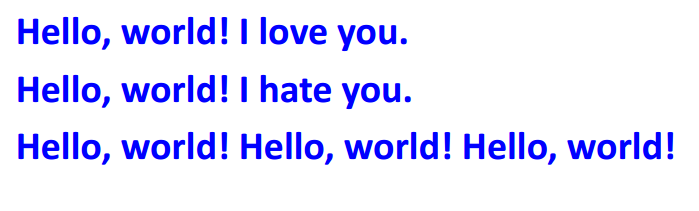
\includegraphics[width=0.5\textwidth]{diagrams/lz77_1.png}\end{figure}
\begin{figure}[H] \caption{Compression starts with literal representation.}
\centering
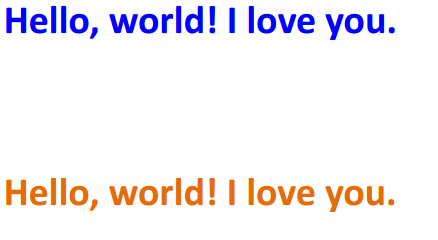
\includegraphics[width=0.35\textwidth]{diagrams/lz77_2.png}\end{figure}
\begin{figure}[H] \caption{We then use a pointer at distance 26 and length 16.}
\centering
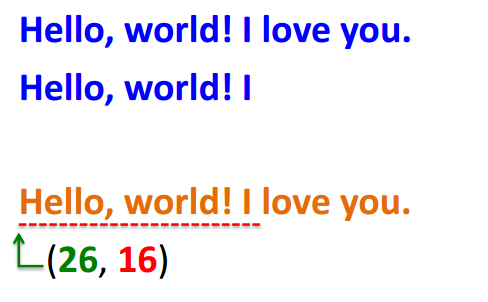
\includegraphics[width=0.35\textwidth]{diagrams/lz77_3.png}\end{figure}
\begin{figure}[H] \caption{We continue with literal.} \centering
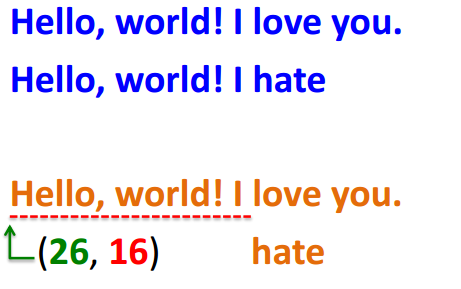
\includegraphics[width=0.35\textwidth]{diagrams/lz77_4.png}\end{figure}
\begin{figure}[H] \caption{We use a pointer pointing to a pointer.} \centering
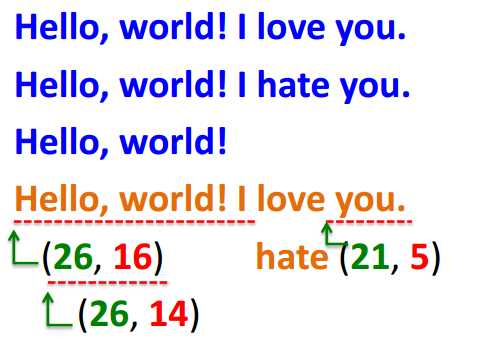
\includegraphics[width=0.35\textwidth]{diagrams/lz77_5.png}\end{figure}
\begin{figure}[H] \caption{We then use a pointer pointing to a pointer pointing
to a pointer.} \centering
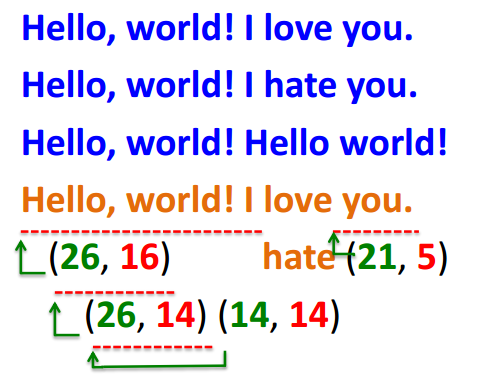
\includegraphics[width=0.35\textwidth]{diagrams/lz77_6.png}\end{figure}
\begin{figure}[H] \caption{Finally, we use a pointer pointing to itself.}
\centering
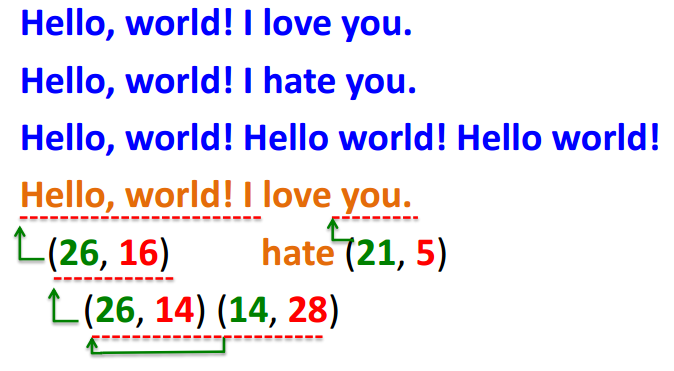
\includegraphics[width=0.5\textwidth]{diagrams/lz77_7.png}\end{figure}


\subsection{Huffman coding} Huffman coding is also a lossless data compression
algorithm developed by David A. Huffman and published in 1952. \cite{huffman}
When compressing a text, a variable-length code table is created to map source
symbols to bitstreams. Each source symbol can be of less or more bits than
originally and the mapping table is used to translate source symbols into
bitstreams during compression and vice versa during decompression. The mapping
table could be represented by a binary tree of nodes. Each leaf node represents
a source symbol, which can be accessed from the root by following the left path
for 0 and the right path for 1. Each source symbol can be represented only by
    leaf nodes, therefore the code is prefix-free, meaning no bitstream
    representing a source symbol can be the prefix of any other bitstream
    representing a different source symbol. The final mapping of source symbols
    to bistreams is calculated by finding the frequency of appearance for each
    source symbol of the plaintext. That way, most common symbols can be coded
    in shorter bitstreams, thus compressing the initial text.

Below follows an example of a plaintext and a valid Huffman tree for compressing
it:

\bigskip \centerline{\textit{\textbf{Chancellor on bring of second bailout for
banks}} \footnote{\url{https://en.bitcoin.it/wiki/Genesis_block}}}

\bigskip \centerline{\textbf{Frequency Analysis}}

\begin{table}[H] \centering \begin{tabular}{ | l | l | l | l | } \hline
\textbf{o}: 6 & \textbf{n}: 5 & \textbf{r}: 3 & \textbf{l}: 3 \\ \textbf{b}: 3 &
\textbf{c}: 3 & \textbf{a}: 3 & \textbf{s}: 2 \\ \textbf{k}: 2 & \textbf{e}: 2 &
\textbf{i}: 2 & \textbf{f}: 2 \\ \textbf{h}: 1 & \textbf{d}: 1 & \textbf{t}: 1 &
\textbf{u}: 1 \\ \hline \end{tabular} \end{table}

\centerline{\textbf{Huffman tree}}

\begin{table}[H] \centering \begin{tabular}{ | l | l | l | l | } \hline
\textbf{o}: 00 & \textbf{n}: 01 & \textbf{r}: 1000 & \textbf{l}: 1001 \\
\textbf{b}: 1010 & \textbf{c}: 1011 & \textbf{a}: 11000 & \textbf{s}: 11001 \\
\textbf{k}: 11010 & \textbf{e}: 11011 & \textbf{i}: 11100 & \textbf{f}: 1111000
\\ \textbf{h}: 1111001 & \textbf{d}: 1111010 & \textbf{t}: 1111011 & \textbf{u}:
1111100 \\ \hline \end{tabular} \end{table}

\centerline{\textbf{Initial text size: 320 bits}} \centerline{\textbf{Compressed
text size: 167 bits}}

\section{Same-origin policy}\label{sec:sameorigin}

Same-origin policy is an important aspect of the web application security model.
According to that policy, a web browser allow scripts contained in one page to
access data in a second page only if both pages have the same \textit{origin}.
Origin is defined as the combination of Uniform Resource Identifier scheme,
hostname and port number. For example, a document retrieved from the website
\textit{http://example.com/target.html} is not allowed under the same-origin
policy to access the Document-Object Model of a document retrieved from
\textit{https://head.example.com/target.html}, since the two websites have
different URI schema (\textit{http} vs \textit{https}) and different hostname
(\textit{example.com} vs \textit{head.example.com}).

Same-origin policy is particularly important in modern web applications, that
rely greatly on HTTP cookies to maintain authenticated sessions. If same-origin
policy was not implemented the data confidentiality and integrity of cookies, as
well as every other content of web pages, would have been compromised. However,
despite the application of same-origin policy by modern browsers, there exist
attacks that enable an adversary to bypass it and breach a user's communication
with a website. Two such major types of vulnerabilities, cross-site scripting
and cross-site request forgery are described in the following subsections.

\subsection{Cross-site scripting}

Cross-site scripting (XSS) is a security vulnerability that allows an adversary
to inject client-side script into web pages viewed by other users. That way,
same-origin policy can be bypassed and sensitive data handled by the vulnerable
website may be compromised. XSS could be divided into two major types,
\textit{non-persistent} and \textit{persistent}
\footnote{\url{https://en.wikipedia.org/wiki/Cross-site_scripting}}, which we
will describe below.

Non-persistent XSS vulnerabilities are the most common. They show up when the
web server does not parse the input in order to escape or reject HTML control
characters, allowing for scripts injected to the input to run unnoticeable.
Usual methods of performing non-persistent XSS include mail or website url links
and search requests.

Persistent XSS occurs when data provided by the attacker are stored by the
server. Responses from the server to different users will then include the
script injected from the attacker, allowing it to run automatically on the
victim's browsers without needing to target them individually. An example of
such attack is when posting texts on social networks or message boards.

\subsection{Cross-site request forgery}

Cross-site request forgery (CSRF) is an exploit that allows an attacker to issue
unauthorized commands to a website, on behalf of a user the website trusts.
Hence the attacker can forge a request to perform actions or post data on a
website the victim is logged in, execute remote code with root privileges or
compromise a root certificate, resulting in a breach of a whole public key
infrastructure (PKI).

CSRF can be performed when the victim is trusted by a website and the attacker
can trick the victim's browser into sending HTTP requests to that website. For
example, when a Alice visits a web page that contains the HTML image tag
\textit{<img
src="\url{http://bank.example.com/withdraw?account=Alice&amount=1000000&for=Mallory}">}
\footnote{\url{https://en.wikipedia.org/wiki/Cross-site_request_forgery}} that
Mallory has injected, a request from Alice's browser to the example bank's
website will be issued, stating for an amount of 1000000 to be transfered from
Alice's account to Mallory's. If Alice is logged in the example bank's website,
the browser will include the cookie containing Alice's authentication
information in the request, making it a valid request for a transfer. If the
website does not perform more sanity checks or further validation from Alice,
the unauthorized transaction will be completed. An attack such as this is very
common on Internet forums that allow users to post images.

A method of mitigation of CSRF is a Cookie-to-Header token. The web application
sets a cookie that contains a random token that validates a specific user
session. Javascript on client side reads that token and includes it in a HTTP
header sent with each request to the web application. Since only Javascript
running within the same origin will be allowed to read the token, we can assume
that it's value is safe from unauthorized scripts to read and copy it to a
custom header in order to mark a rogue request as valid.

\section{Transport Layer Security}\label{sec:tls}

Transport Layer Security (TLS) is a protocol that provides communications
security over the internet, allowing a server and a client to communicate in a
way that prevents eavesdropping, tampering or message forgery. \cite{tls12}

The users negotiate a symmetric key via assymetric cryptography that is provided
by X.509 certificates, therefore there exist certificate authorities and a
public key infrastructure (PKI), in order for the certificates to be verified
for their owners. However, it can be understood that, due to their key role,
    certificate authorities are points of failure in the system, enabling for
    Man-in-the-Middle attacks, in a case when an adversary has managed to forge
    a root certificate.

Apart from certificate-related attacks, a well-known category is compression
attacks. \footnote{\url{https://tools.ietf.org/html/rfc7457}} Such attacks
exploit TLS-level compression so as to decrypt ciphertext. In this document, we
investigate the threat model and performance of such an attack,
\href{http://breachattack.com}{BREACH}.

In the following subsections we will briefly describe some of the protocol
details, especially handshake and the format of TLS records.

\subsection{TLS handshake}

\begin{figure}[H] \caption{TLS handshake flow.} \centering
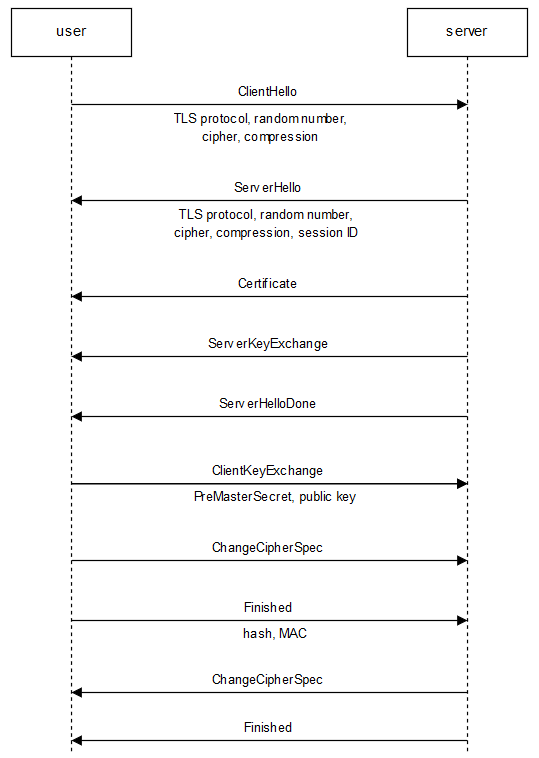
\includegraphics[width=0.7\textwidth]{diagrams/tls_handshake.png}\end{figure}

This sequence diagram presents the functionality of TLS handshake. User and
server exchange the basic parameters of the connection, specifically the
protocol version, cipher suite, compression method and random numbers, with the
ClientHello and ServerHello records. The server then provides all information
needed from the user to validate and use the asymmetric server key, in order to
compute the symmetric key to be used in the rest of the communication. The
client computes a \textit{PreMasterKey}, that is sent to the server, which is
used by both parties to compute the symmetric key. Finally, both sides exchange
and validate hash and MAC over the previous messages, after which they both have
the ability to communicate safely.

The above flow describes the basic TLS handshake. Client-authenticated and
resumed handshakes have similar functionality, which are not relevant for the
purpose of this paper.

\subsection{TLS record}

\begin{figure}[H] \caption{TLS record.} \centering
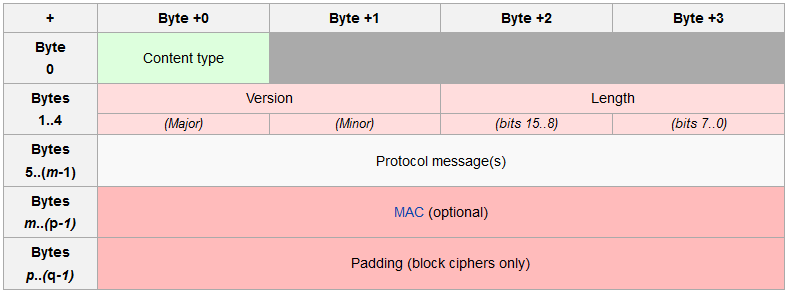
\includegraphics[width=1\textwidth]{diagrams/tls_record.png}\end{figure}

The above figure
\footnote{\url{https://en.wikipedia.org/wiki/Transport_Layer_Security}} depicts
the general format of all TLS records.

The first field describes the Record Layer Protocol Type contained in the
record, which can be one of the following:

\begin{table}[H] \centering \begin{tabular}{ | l | l | } \hline \textbf{Hex} &
\textbf{Type} \\ \hline 0x14 & ChangeCipherSpec \\ 0x15 & Alert \\ 0x16 &
Handshake \\ 0x17 & Appliation \\ 0x18 & Heartbeat \\ \hline \end{tabular}
\end{table}

The second field defines the TLS version for the record message, which is
identified my the major and minor version as below:

\begin{table}[H] \centering \begin{tabular}{ | l | l | l | } \hline
\textbf{Major} & \textbf{Minor} & \textbf{Version} \\ \hline 3 & 0 & SSL 3.0 \\
3 & 1 & TLS 1.0 \\ 3 & 2 & TLS 1.1 \\ 3 & 3 & TLS 1.2 \\ \hline \end{tabular}
\end{table}

The length of the contained record message, MAC and padding is then calculated
by the following two fiels as: \begin{math}256*(bits 15..8) + (bits
7..0)\end{math}.

Finally, the payload of the record, which, depending on the type, may be
encrypted, the MAC, if provided, and the padding, if needed, make up the rest of
the TLS record.

\section{Man-in-the-Middle}\label{sec:mitm}

Man-in-the-Middle (MitM) is one of the most common attack vectors, where an
attacker reroutes the communication of two parties, in order to be controlled
and possibly altered. The aggressiveness of the attack can vary from passive
eavesdropping to full control of the communication, as long as the attacker is
able to impersonate both parties and convince them to be trusted.

\begin{figure}[H] \caption{Man-in-the-Middle.} \centering
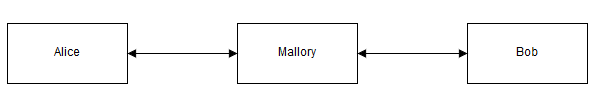
\includegraphics[width=1\textwidth]{diagrams/mitm.png}\end{figure}

MitM attacks can be mitigated by using end-to-end cryptography, mutual
authentication or PKIs. However, some attacks manage to bypass such mitigation
techniques. Below, we descripe two such attacks, ARP Spoofing and DNS cache
poisoning.

\subsection{ARP Spoofing} ARP spoofing
\footnote{\url{https://en.wikipedia.org/wiki/ARP_spoofing}} is a technique where
an attacker sends Address Resolution Protocol (ARP) messages over the network,
so as to assosiate the MAC address with the IP address of another host. That
way, the attacker may intercept the traffic of the network, modify or deny
packets, performing denial of service, MitM or session hijacking attacks.

\begin{figure}[H] \caption{Arp Spoofing.} \centering
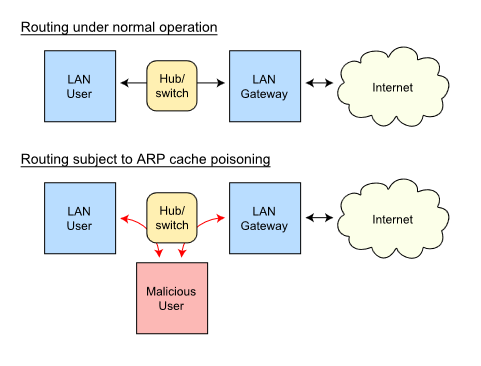
\includegraphics[width=0.8\textwidth]{diagrams/arp_spoofing.png}\end{figure}

ARP spoofing can be also used for legitimate reasons, when a developer needs to
debug IP traffic between two hosts. That way, the developer can act as proxy
between the two hosts or configure the switch that is normally used by the two
parties to forward traffic for monitoring.

\subsection{DNS spoofing}

\begin{figure}[H] \caption{DNS Spoofing.} \centering
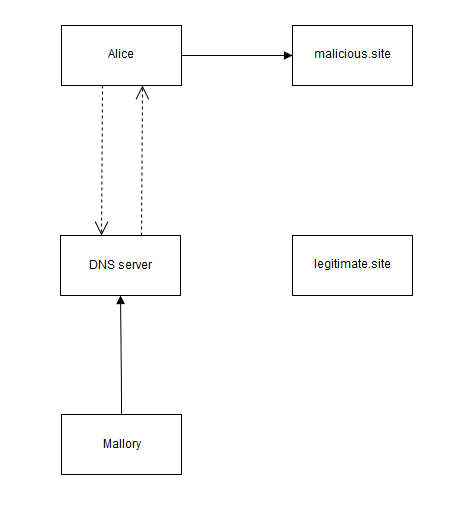
\includegraphics[width=0.5\textwidth]{diagrams/dns_spoofing.png}\end{figure}

DNS spoofing (or DNS cache poisoning) is an attack, when the adversary
introduces data into a Domain Name System resolver's cache, in order to return
an incorrect address for a specific host.

DNS servers are usually provided by Internet Service Providers (ISPs), used to
resolve IP addresses to human-readable hostnames faster. A malicious employee,
or anyone that has gained unauthorized access to the server, can then perform
DNS poisoning, affecting every user that is being serviced by that server.
